\documentclass[multi=tikzpicture, border=1cm]{standalone}
\usepackage{pgfplots, tikz-3dplot}
\usetikzlibrary{decorations.text, decorations.markings}
\usetikzlibrary{intersections}
\usetikzlibrary{arrows.meta}
\usetikzlibrary{shapes, shadows}
\usetikzlibrary{quotes,angles}
\pgfdeclarelayer{bg}    % declare background layer
\pgfsetlayers{bg,main}  % set the order of the layers (main is the standard layer)
\usetikzlibrary{shapes.geometric,calc}
\usepgfplotslibrary{fillbetween}
\pgfplotsset{
	every axis label/.append style={font=\small},
	compat=newest,
}
\tikzset{every picture/.style={font=\small}}
% -------------------------------------- Електричні кола ------------------------------------------------
\usetikzlibrary{circuits.ee.IEC}
\tikzset{circuit ee IEC,
every info/.style=red,
semithick,
every info/.style={font=\footnotesize},
small circuit symbols,
circuit declare symbol = ampermeter,
circuit declare symbol = voltmeter,
circuit declare symbol = galvanometer,
set ampermeter graphic = {draw,generic circle IEC, minimum size=5mm,info=center:A},%
set voltmeter graphic = {draw,generic circle IEC, minimum size=5mm,info=center:V},
set galvanometer graphic = {draw,generic circle IEC, minimum size=5mm,info=center:G},
}

% -------------------------------------- Grid -------------------------------------------------------
\makeatletter
\def\grd@save@target#1{%
  \def\grd@target{#1}}
\def\grd@save@start#1{%
  \def\grd@start{#1}}
\tikzset{
  grid with coordinates/.style={
    to path={%
      \pgfextra{%
        \edef\grd@@target{(\tikztotarget)}%
        \tikz@scan@one@point\grd@save@target\grd@@target\relax
        \edef\grd@@start{(\tikztostart)}%
        \tikz@scan@one@point\grd@save@start\grd@@start\relax
        \draw[minor help lines] (\tikztostart) grid (\tikztotarget);
        \draw[major help lines] (\tikztostart) grid (\tikztotarget);
        \grd@start
        \pgfmathsetmacro{\grd@xa}{\the\pgf@x/1cm}
        \pgfmathsetmacro{\grd@ya}{\the\pgf@y/1cm}
        \grd@target
        \pgfmathsetmacro{\grd@xb}{\the\pgf@x/1cm}
        \pgfmathsetmacro{\grd@yb}{\the\pgf@y/1cm}
        \pgfmathsetmacro{\grd@xc}{\grd@xa + \pgfkeysvalueof{/tikz/grid with coordinates/major step}}
        \pgfmathsetmacro{\grd@yc}{\grd@ya + \pgfkeysvalueof{/tikz/grid with coordinates/major step}}
        \foreach \x in {\grd@xa,\grd@xc,...,\grd@xb}
        \node[anchor=north] at (\x,\grd@ya) {\pgfmathprintnumber{\x}};
        \foreach \y in {\grd@ya,\grd@yc,...,\grd@yb}
        \node[anchor=east] at (\grd@xa,\y) {\pgfmathprintnumber{\y}};
      }
    }
  },
  minor help lines/.style={
    help lines,
    step=\pgfkeysvalueof{/tikz/grid with coordinates/minor step}
  },
  major help lines/.style={
    help lines,
    line width= 0.5pt,
    step=\pgfkeysvalueof{/tikz/grid with coordinates/major step}
  },
  grid with coordinates/.cd,
  minor step/.initial=.2,
  major step/.initial=1,
  major line width/.initial=2pt,
}
\makeatother
% ------------------------------------ Паттерни -----------------------------------------------------
\usetikzlibrary{patterns}
\tikzstyle{ground}=[fill,pattern=north east lines,draw=none,minimum width=0.3,minimum height=0.6]

% ------------------------------------ Молекулярний струм -------------------------------------------
% #1,#2 - центр; #3 - кут напряму дипольного моменту (град.)
% контур лежить у площині, перпендикулярній до моменту;
% стрілка моменту виходить з центра кільця вздовж нормалі
\newcommand{\ampere}[3]{%
  \begin{scope}[shift={(#1,#2)},rotate=#3]
    \draw[magenta!80!purple,thick] (0,0) ellipse [x radius=.3,y radius=.5];
    \draw[magenta!80!purple,thick,-{Stealth[length=2.2mm]}]
      ({.3*cos(170)},{.5*sin(170)})
      arc [start angle=170,end angle=195,x radius=.3,y radius=.5];
    \draw[black,thick,-{Stealth[length=3mm]}] (0,0) -- (.8,0);
  \end{scope}%
}

\begin{document}

% ======================= Рис. 1. Намагнічений стрижень =======================
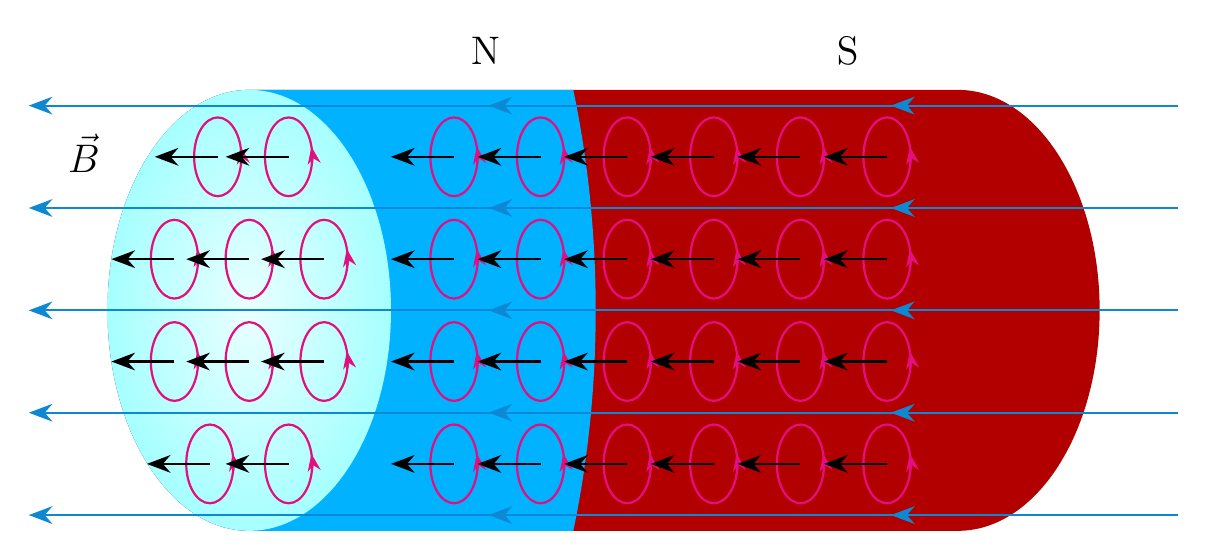
\begin{tikzpicture}
  \def\ra{1.8}\def\rb{2.8}\def\LL{9}
  \def\body{(0,\rb) -- (\LL,\rb)
    arc [start angle=90,end angle=-90,x radius=\ra,y radius=\rb] -- (0,-\rb)
    arc [start angle=270,end angle=90,x radius=\ra,y radius=\rb] -- cycle}

  % тіло: спочатку червона частина (S), поверх неї синя (N)
  \begin{scope}
    \clip \body;
    \shade[top color=red!70!black,middle color=red!45!white,bottom color=red!70!black]
      (-3,-\rb) rectangle (\LL+3,\rb);
    \begin{scope}
      \clip (-3,4) -- (3.8,4) .. controls (4.6,1.5) and (4.6,-1.5) .. (3.8,-4) -- (-3,-4) -- cycle;
      \shade[top color=cyan!70!blue,middle color=cyan!40!white,bottom color=cyan!70!blue]
        (-3,-\rb) rectangle (\LL+3,\rb);
    \end{scope}
  \end{scope}

  % молекулярні струми в товщі матеріалу (усі моменти вліво, вздовж B)
  \foreach \x in {2.6,3.7,...,8.1}
    \foreach \y in {1.95,0.65,-0.65,-1.95}
      {\ampere{\x}{\y}{180}}

  % торцева грань
  \shade[inner color=cyan!8,outer color=cyan!35]
    (0,0) ellipse [x radius=\ra,y radius=\rb];

  % поле B: пронизує весь стрижень, у тому числі торець; напрям S -> N (вліво)
  \foreach \y in {-2.6,-1.3,0,1.3,2.6}
    \draw[cyan!70!blue,thick,-{Stealth[length=3mm]},
          postaction={decorate},
          decoration={markings,
            mark=at position 0.25 with {\arrow{Stealth[length=3mm]}},
            mark=at position 0.6 with {\arrow{Stealth[length=3mm]}}}]
      (\LL+\ra+1,\y) -- (-2.8,\y);

  % молекулярні струми з однаково напрямленими моментами (вздовж B, вліво)
  \foreach \x/\y in {-0.4/1.95, 0.5/1.95,
                     -0.95/0.65, 0/0.65, 0.95/0.65,
                     -0.95/-0.65, 0/-0.65, 0.95/-0.65,
                     -0.5/-1.95, 0.5/-1.95}
    {\ampere{\x}{\y}{180}}

  \node at (-2.1,2.0) {\Large $\vec B$};
  \node at (3.0,3.3) {\Large N};
  \node at (7.6,3.3) {\Large S};
\end{tikzpicture}

% ======================= Рис. 2. Ненамагнічений стрижень =======================
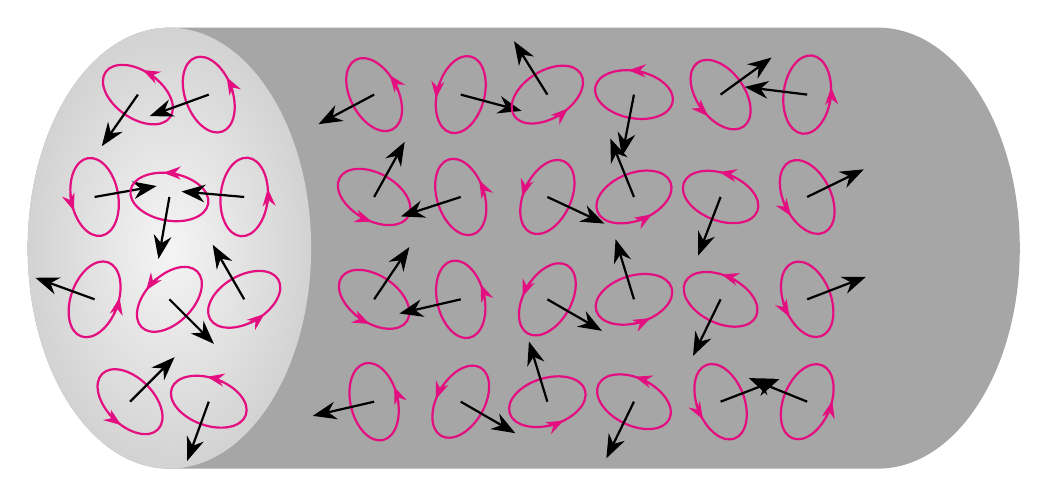
\begin{tikzpicture}
  \def\ra{1.8}\def\rb{2.8}\def\LL{9}
  \def\body{(0,\rb) -- (\LL,\rb)
    arc [start angle=90,end angle=-90,x radius=\ra,y radius=\rb] -- (0,-\rb)
    arc [start angle=270,end angle=90,x radius=\ra,y radius=\rb] -- cycle}

  \begin{scope}
    \clip \body;
    \shade[top color=gray!70,middle color=gray!12,bottom color=gray!70]
      (-3,-\rb) rectangle (\LL+3,\rb);
  \end{scope}

  % молекулярні струми в товщі: детерміновано «випадкові» напрями
  \foreach \x [count=\i] in {2.6,3.7,...,8.1}
    \foreach \y [count=\j] in {1.95,0.65,-0.65,-1.95}
      {\pgfmathsetmacro{\m}{mod(137*\i+71*\j*\j,360)}
       \ampere{\x}{\y}{\m}}

  \shade[inner color=gray!8,outer color=gray!35]
    (0,0) ellipse [x radius=\ra,y radius=\rb];

  % хаотичні напрями: x / y / кут напряму дипольного моменту
  \foreach \x/\y/\m in {-0.4/1.95/235,  0.5/1.95/200,
                        -0.95/0.65/10, 0/0.65/260, 0.95/0.65/175,
                        -0.95/-0.65/160, 0/-0.65/315, 0.95/-0.65/120,
                        -0.5/-1.95/45, 0.5/-1.95/250}
    {\ampere{\x}{\y}{\m}}
\end{tikzpicture}

\end{document}